Configure both the office computer and the home computer according to the following specifications. You can find instructions for such a scenario at

http://www.openvpn.net

to view. Determine which standard encryption OpenVPN uses, answer the following questions
whether this method is still up-to-date or secure and indicate how you can switch to a more secure method.
to a more secure method.

\begin{figure}[H]
	\centering
	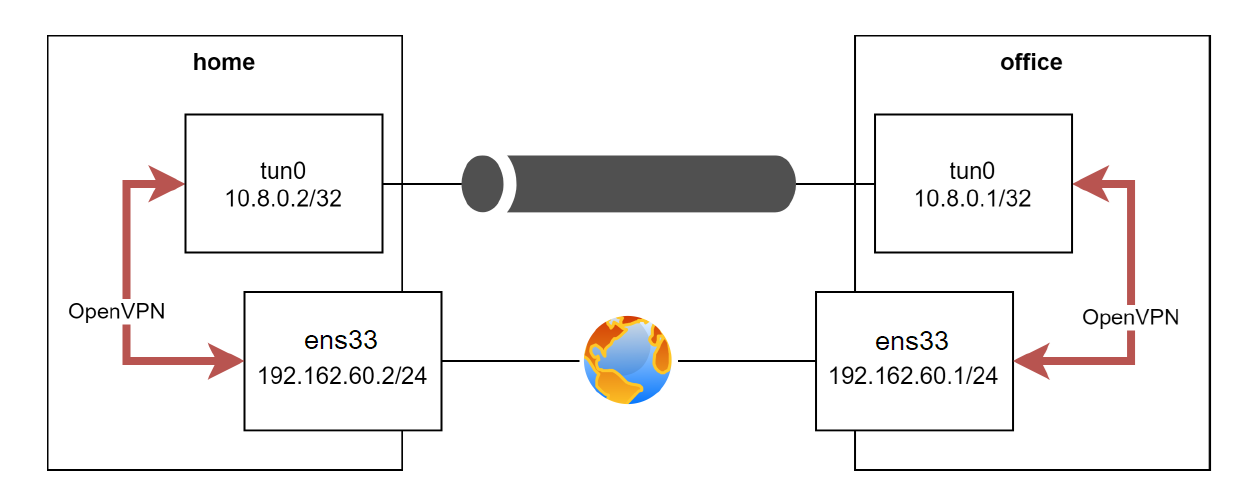
\includegraphics[width=0.8\linewidth]{Figures/home-office.png}
	\caption{Home - Office Network}
\end{figure}

To set the static IP address, of both computers we used netplan, here is the config from the office computer:

\begin{minted}{yaml}
root@ntsi:/etc/netplan# cat 00-config.yaml 
network:
    version: 2
    renderer: NetworkManager
    ethernets:
    ens33:
        dhcp4: no
        addresses:
        - 192.168.60.1/24
\end{minted}

Then we used the command netplan apply to apply the changes. The home computer has the same configuration, except for the IP address, which is 192.168.60.2.
\\\\
Here is the OpenVPN configuration of the home computer with an explanation after every line, in /etc/openvpn/home\.conf:

\begin{minted}{text}
dev tun0 # Uses a tun interface named tun0 for the VPN tunnel
proto udp # Uses UDP for the underlying transport protocol (default in OpenVPN)
ifconfig 10.8.0.2 10.8.0.1 # Sets local IP of the tun0 to 10.8.0.2, remote to 10.8.0.1
remote 192.168.60.1 1194 # Connects remote at IP 192.168.60.1 on port 1194
secret keys/static.key # Uses PSK located at keys/static
cipher AES-256-CBC # Sets the encryption cipher to AES-256 CBC
\end{minted}

Here for the office computer, in /etc/openvpn/office\.conf:

\begin{minted}{text}
dev tun0 # Uses a tun interface named tun0 for the VPN tunnel
proto udp # Uses UDP for the underlying transport protocol (default in OpenVPN)
ifconfig 10.8.0.1 10.8.0.2 # Sets local IP of the tun0 to 10.8.0.1, remote to 10.8.0.2
secret keys/static.key # Uses PSK located at keys/static
port 1194 # Listens for incoming connections on port 1194
cipher AES-256-CBC # Sets the encryption cipher to AES-256 CBC
\end{minted}
AES-256-CBC has to be set manually, otherwise you get the following error message:

\begin{minted}{text}
2024-12-29 18:15:07 Cipher BF-CBC not supported
2024-12-29 18:15:07 Exiting due to fatal error
\end{minted}


The keys were generated using the following command:

\begin{minted}{bash}
openvpn --genkey --secret static.key
\end{minted}

This is the entire connection buildup and breakdown process:

\begin{minted}{bash}
root@ntsi:/etc/openvpn# openvpn --config home.conf
2024-12-29 18:07:31 DEPRECATED OPTION: The option --secret is deprecated.
2024-12-29 18:07:31 DEPRECATION: No tls-client or tls-server option in configuration detected. OpenVPN 2.7 will remove the functionality to run a VPN without TLS. See the examples section in the manual page for examples of a similar quick setup with peer-fingerprint.
2024-12-29 18:07:31 OpenVPN 2.6.9 x86_64-pc-linux-gnu [SSL (OpenSSL)] [LZO] [LZ4] [EPOLL] [PKCS11] [MH/PKTINFO] [AEAD] [DCO]
2024-12-29 18:07:31 library versions: OpenSSL 3.0.13 30 Jan 2024, LZO 2.10
2024-12-29 18:07:31 DCO version: N/A
2024-12-29 18:07:31 TUN/TAP device tun0 opened
2024-12-29 18:07:31 net_iface_mtu_set: mtu 1500 for tun0
2024-12-29 18:07:31 net_iface_up: set tun0 up
2024-12-29 18:07:31 net_addr_ptp_v4_add: 10.8.0.2 peer 10.8.0.1 dev tun0
2024-12-29 18:07:31 TCP/UDP: Preserving recently used remote address: [AF_INET]192.168.60.1:1194
2024-12-29 18:07:31 UDPv4 link local (bound): [AF_INET][undef]:1194
2024-12-29 18:07:31 UDPv4 link remote: [AF_INET]192.168.60.1:1194
2024-12-29 18:07:31 read UDPv4 [ECONNREFUSED]: Connection refused (fd=4,code=111)
2024-12-29 18:07:35 read UDPv4 [ECONNREFUSED]: Connection refused (fd=4,code=111)
2024-12-29 18:07:41 read UDPv4 [ECONNREFUSED]: Connection refused (fd=4,code=111)
2024-12-29 18:07:42 read UDPv4 [ECONNREFUSED]: Connection refused (fd=4,code=111)
2024-12-29 18:07:56 read UDPv4 [ECONNREFUSED]: Connection refused (fd=4,code=111)
2024-12-29 18:08:02 read UDPv4 [ECONNREFUSED]: Connection refused (fd=4,code=111)
2024-12-29 18:08:12 Peer Connection Initiated with [AF_INET]192.168.60.1:1194
2024-12-29 18:08:13 Initialization Sequence Completed
^C2024-12-29 18:08:18 event_wait : Interrupted system call (fd=-1,code=4)
2024-12-29 18:08:18 net_addr_ptp_v4_del: 10.8.0.2 dev tun0
2024-12-29 18:08:18 SIGINT[hard,] received, process exiting
\end{minted}

The connection refused messages are because the office computer was not running the OpenVPN server at that time. The connection was established after the server was started. The connection was then closed by pressing Ctrl+C. The connection was established successfully, as shown by the "Initialization Sequence Completed" message.
\\\\
Before OpenVPN version 2.5 the default encryption cipher was Blowfish in CBC mode (BF-CBC).

OpenVPN version 2.5 introduced Negotiable Cipher Parameters (NCP), OpenVPN will try to use AES-256-GCM or AES-128-GCM by default if the negotiated cipher parameters (NCP) feature is enabled and both sides have a compatible cipher in their allowed list. If NCP is disabled or a common cipher can not be found, it will fall back to BF-CBC.